%%%%%%%%%%%%%%%%%%%%%%%%%%
%%% author : Yamada. T %%%
%%% made for TH series %%%
%%%%%%%%%%%%%%%%%%%%%%%%%%

\documentclass[b5paper,10pt,fleqn] {ltjsarticle}

\usepackage[margin=10truemm]{geometry}

\usepackage{pict2e, graphicx}
\usepackage{tikz}
\usetikzlibrary{intersections,calc,arrows.meta}

\usepackage{amsmath, amssymb, amsthm}
\usepackage{ascmac}
\usepackage{comment}
\usepackage{empheq}
\usepackage[shortlabels,inline]{enumitem}
\usepackage{fancybox}
\usepackage{fancyhdr}
\usepackage{here}
\usepackage{lastpage}
\usepackage{listings, jvlisting}
\usepackage{fixdif}

\usepackage{stmaryrd}
\usepackage[listings]{tcolorbox}
%\usepackage{ascolorbox}
\usepackage{titlesec}
\usepackage{ulem}
\usepackage{url}
\usepackage{verbatim}
\usepackage{wrapfig}
\usepackage{xcolor}
\usepackage{luatexja-ruby}
\usepackage{varwidth}
\usepackage[version=3]{mhchem}
\usepackage{wrapfig}


\usepackage{physics2}
	\usephysicsmodule{ab}
	\usephysicsmodule{ab.braket}
	\usephysicsmodule{ab.legacy}
	%\usephysicsmodule{braket}
	\usephysicsmodule{diagmat}
	\usephysicsmodule{xmat}
	\usephysicsmodule{nabla.legacy}
	\usephysicsmodule{qtext.legacy}

\usepackage[ISO]{diffcoeff}
\difdef { f, s } { D }
{ op-symbol = \mathrm{D} }


\newcommand{\mctext}[1]{\mbox{\textcircled{\scriptsize{#1}}}}
\newcommand{\ctext}[1]{\textcircled{\scriptsize{#1}}}
\newcommand{\ds}{\displaystyle}
\newcommand{\comb}[2]{{}_{#1}\mathrm{C}_{#2}}
\newcommand{\hs}{\hspace}
\newcommand{\vs}{\vspace}
\newcommand{\emphvs}{\vspace{1em}\notag\\}
\newcommand{\ora}{\overrightarrow}
\newcommand{\ol}{\overline}
\newcommand{\oramr}[1]{\overrightarrow{\mathrm{#1}}}
\newcommand{\tri}{\triangle}
\newcommand{\mr}{\mathrm}
\newcommand{\mb}{\mathbb}
\newcommand{\mrvec}[1]{\overrightarrow{\mathrm{#1}}}
\newcommand{\itvec}{\overrightarrow}
\newcommand{\bs}{\boldsymbol}
\newcommand{\ra}{\rightarrow}
\newcommand{\Ra}{\Rightarrow}
\newcommand{\lra}{\longrightarrow}
\newcommand{\Lra}{\Longrightarrow}
\newcommand{\la}{\leftarrow}
\newcommand{\La}{\Leftarrow}
\newcommand{\lla}{\longleftarrow}
\newcommand{\Lla}{\Longleftarrow}
\newcommand{\lr}{\leftrightarrow}
\newcommand{\llr}{\longleftrightarrow}
\newcommand{\Llr}{\Longleftrightarrow}
\renewcommand{\deg}{{}^\circ}
\newcommand{\phbox}{\fbox{\phantom{1\hspace{2em}}}}
\newcommand{\boxnum}[1]{\fbox{\phantom{\hspace{1em}}({#1})\phantom{\hspace{1em}}}}
\newcommand{\boxkana}[1]{\fbox{\phantom{\hspace{1em}}{#1}\phantom{\hspace{1em}}}}
\newcommand{\boxkm}[2]{\fbox{\, {#1}\phantom{\hspace{0.2em}} \,  {#2}}}
\newcommand{\hzw}{\hspace{1\zw}}

\renewcommand{\baselinestretch}{1.25}
\parindent=1\zw

%入95
\begin{document}
\noindent
\fbox{NewTH1-12} [東京大]


図1のように,ばね定数$k$を持つばねが階段上に等間隔に並んでいる.
隣り合ったばねの水平方向の間隔を$w$とする.
ばねの上には質量$M$の板が固定されている.
ばねの長さはどれも等しく,ばねの質量は無視できる.
ばねは鉛直方向の振動だけが許されている.
隣り合った板の平衡位置の高さの差を$h$とする.
また,重力加速度の大きさを$g$とする.

\begin{figure}[H]
  \centering
  \begin{minipage}{0.45\linewidth}
  \centering
  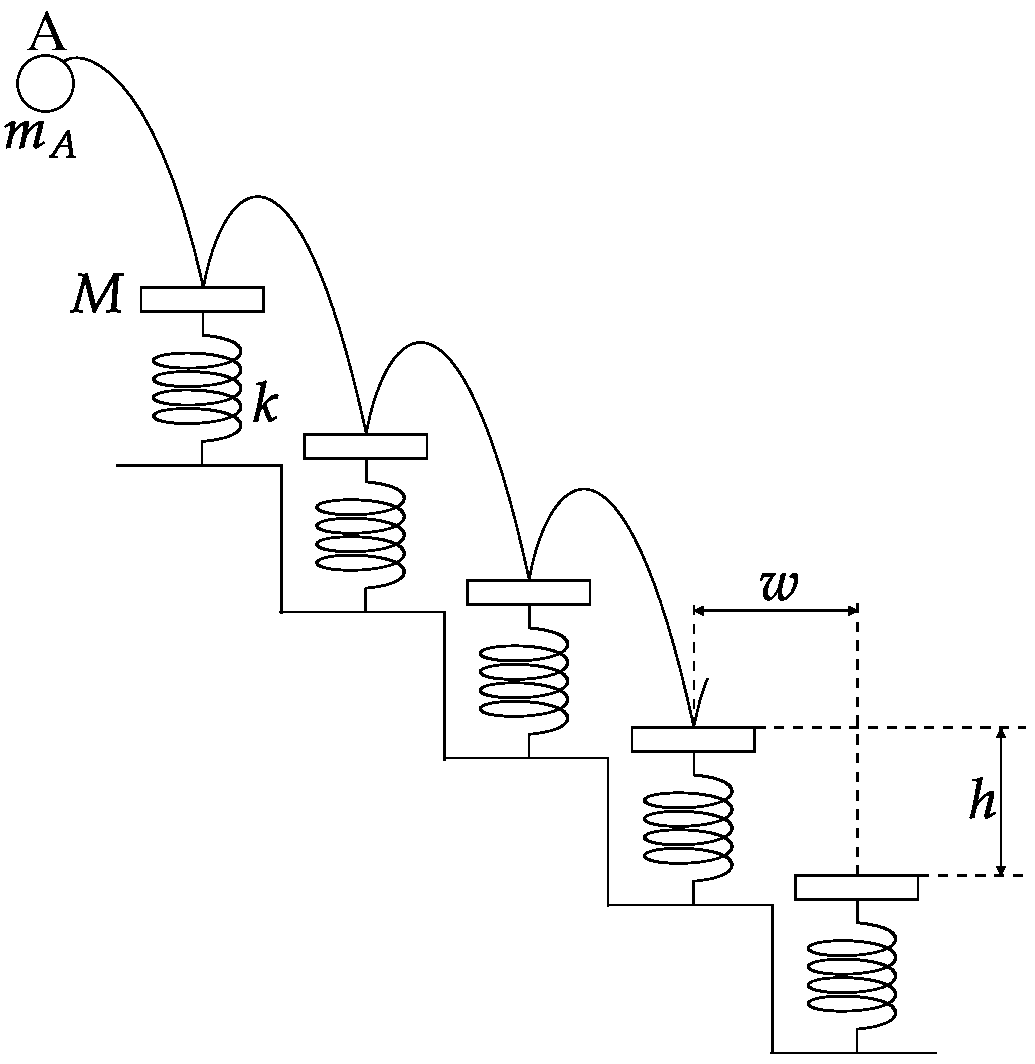
\includegraphics[width=6cm]{fig/fig_1_12_1.pdf}

  \vspace{-1cm}
  図1
  \end{minipage}
  \begin{minipage}{0.45\linewidth}
  \centering
  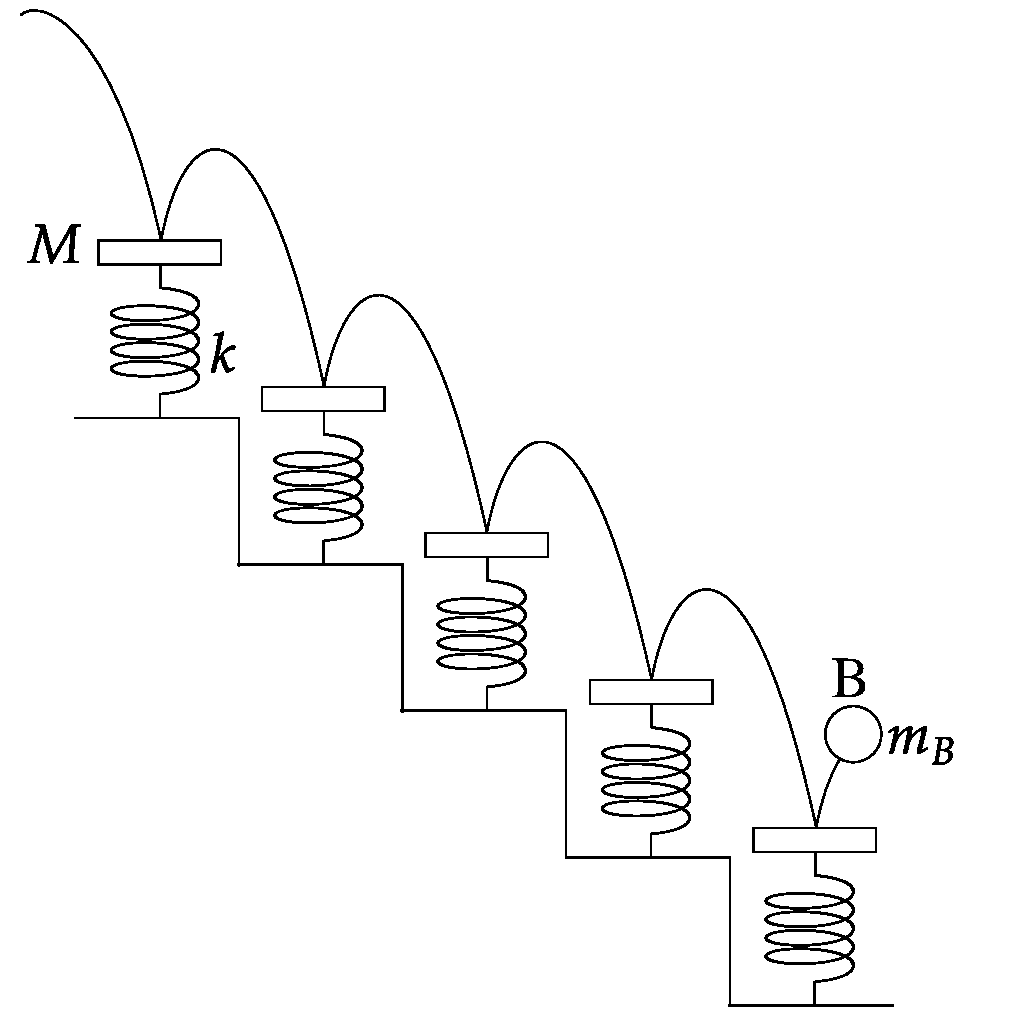
\includegraphics[width=6cm]{fig/fig_1_12_2.pdf}
  
  \vspace{-1cm}
  図2
  \end{minipage}
\end{figure}

\begin{enumerate}[I]
  \item {\hzw}すべての板を平衡位置に静止させ,質量$m_\mr{A}$を持つ物体A(質点)を階段上方のある位置からある初速度で運動させたところ,Aは図1のように,各板の中心と次々に衝突しながら階段の下方へ運動を続けた.ただし,Aと板は反発係数1で衝突するとし,$M > m_\mr{A}$とする.このとき,以下の設問に答えよ.
  \begin{enumerate}[(1)]
    \item {\hzw}Aが板と衝突する直前において,Aの速度の水平成分を$u$,鉛直成分を$-v$とする(速度の鉛直成分は上方を正とする).このとき,衝突直後のAの速度の鉛直成分を$v$,$m_\mr{A}$,$M$を用いて表せ.
    \item {\hzw}Aが各板の中心と次々に衝突するためには,各衝突直前におけるAの速度は等しくなければならない.この条件を満たす$v$を$m_\mr{A}$,$M$.$h$,$g$を用いて表せ.また,衝突から次の衝突までの時間間隔を$m_\mr{A}$,$M$,$h$,$g$を用いて表せ.
    \item {\hzw}Aが各板の中心と次々に衝突するためには,$u$もある条件を満たす必要がある.そのような$u$を$m_\mr{A}$,$M$,$h$,$g$,$w$を用いて表せ.
    \item {\hzw}Aと衝突した直後に板が持つ運動エネルギーを$m_\mr{A}$,$h$,$g$を用いて表せ.
    \item {\hzw}衝突後,板は単振動を始める.その周期と振幅を$m_\mr{A}$,$M$,$h$,$g$,$k$のうち,必要なものを用いて表せ.
  \end{enumerate}
  \item {\hzw}Aが通り過ぎた後,各板は単振動を続けている.そこで質量$m_\mr{B}$を持つ物体B(質点)を,ある時刻に階段下方のある位置からある初速度で運動させたところ,Bは図2のように各板の中心と次々に衝突しながら階段の上方へ運動を続けた.Bは板と反発係数1で衝突するとし,以下の設問に答えよ.
  \begin{enumerate}[(1)]
    \item {\hzw}Bが図2のような運動をするためには,各衝突直前におけるBの速度は等しくなければならない.また,板についても同様である.したがって,衝突直前における板の振動の位相はどの衝突においても等しくなければならず,衝突から次の衝突までの時間間隔$T$はとびとびの値しか取りえない.その値$T$を$m_\mr{A}$,$M$,$h$,$g$,$k$を用いて表せ.
    \item {\hzw}各衝突の直前と直後における板の速度の鉛直成分を,それぞれ$m_\mr{B}$,$M$,$h$,$g$,$T$を用いて表せ.
    \item {\hzw}各衝突によってBが獲得する力学的エネルギーを$m_\mr{B}$,$h$,$g$を用いて表せ.
    \item {\hzw}$m_\mr{B} > m_\mr{A}$のとき,図2のような運動は起こりえない.その理由を述べよ.
  \end{enumerate}
\end{enumerate}
\end{document}
